\documentclass[11pt,compress,t,notes=noshow, xcolor=table]{beamer}
\usepackage[]{graphicx}\usepackage[]{color}
% maxwidth is the original width if it is less than linewidth
% otherwise use linewidth (to make sure the graphics do not exceed the margin)
\makeatletter
\def\maxwidth{ %
  \ifdim\Gin@nat@width>\linewidth
    \linewidth
  \else
    \Gin@nat@width
  \fi
}
\makeatother

\definecolor{fgcolor}{rgb}{0.345, 0.345, 0.345}
\newcommand{\hlnum}[1]{\textcolor[rgb]{0.686,0.059,0.569}{#1}}%
\newcommand{\hlstr}[1]{\textcolor[rgb]{0.192,0.494,0.8}{#1}}%
\newcommand{\hlcom}[1]{\textcolor[rgb]{0.678,0.584,0.686}{\textit{#1}}}%
\newcommand{\hlopt}[1]{\textcolor[rgb]{0,0,0}{#1}}%
\newcommand{\hlstd}[1]{\textcolor[rgb]{0.345,0.345,0.345}{#1}}%
\newcommand{\hlkwa}[1]{\textcolor[rgb]{0.161,0.373,0.58}{\textbf{#1}}}%
\newcommand{\hlkwb}[1]{\textcolor[rgb]{0.69,0.353,0.396}{#1}}%
\newcommand{\hlkwc}[1]{\textcolor[rgb]{0.333,0.667,0.333}{#1}}%
\newcommand{\hlkwd}[1]{\textcolor[rgb]{0.737,0.353,0.396}{\textbf{#1}}}%
\let\hlipl\hlkwb

\usepackage{framed}
\makeatletter
\newenvironment{kframe}{%
 \def\at@end@of@kframe{}%
 \ifinner\ifhmode%
  \def\at@end@of@kframe{\end{minipage}}%
  \begin{minipage}{\columnwidth}%
 \fi\fi%
 \def\FrameCommand##1{\hskip\@totalleftmargin \hskip-\fboxsep
 \colorbox{shadecolor}{##1}\hskip-\fboxsep
     % There is no \\@totalrightmargin, so:
     \hskip-\linewidth \hskip-\@totalleftmargin \hskip\columnwidth}%
 \MakeFramed {\advance\hsize-\width
   \@totalleftmargin\z@ \linewidth\hsize
   \@setminipage}}%
 {\par\unskip\endMakeFramed%
 \at@end@of@kframe}
\makeatother

\definecolor{shadecolor}{rgb}{.97, .97, .97}
\definecolor{messagecolor}{rgb}{0, 0, 0}
\definecolor{warningcolor}{rgb}{1, 0, 1}
\definecolor{errorcolor}{rgb}{1, 0, 0}
\newenvironment{knitrout}{}{} % an empty environment to be redefined in TeX

\usepackage{alltt}
\newcommand{\SweaveOpts}[1]{}  % do not interfere with LaTeX
\newcommand{\SweaveInput}[1]{} % because they are not real TeX commands
\newcommand{\Sexpr}[1]{}       % will only be parsed by R



\usepackage[english]{babel}
\usepackage[utf8]{inputenc}

\usepackage{dsfont}
\usepackage{verbatim}
\usepackage{amsmath}
\usepackage{amsfonts}
\usepackage{bm}
\usepackage{csquotes}
\usepackage{multirow}
\usepackage{longtable}
\usepackage{booktabs}
\usepackage{enumerate}
\usepackage[absolute,overlay]{textpos}
\usepackage{psfrag}
\usepackage{algorithm}
\usepackage{algpseudocode}
\usepackage{eqnarray}
\usepackage{arydshln}
\usepackage{tabularx}
\usepackage{placeins}
\usepackage{tikz}
\usepackage{setspace}
\usepackage{colortbl}
\usepackage{mathtools}
\usepackage{wrapfig}
\usepackage{bm}
\usetikzlibrary{shapes,arrows,automata,positioning,calc,chains,trees, shadows}
\tikzset{
  %Define standard arrow tip
  >=stealth',
  %Define style for boxes
  punkt/.style={
    rectangle,
    rounded corners,
    draw=black, very thick,
    text width=6.5em,
    minimum height=2em,
    text centered},
  % Define arrow style
  pil/.style={
    ->,
    thick,
    shorten <=2pt,
    shorten >=2pt,}
}
\usepackage{subfig}


% Defines macros and environments

% basic latex stuff
\newcommand{\pkg}[1]{{\fontseries{b}\selectfont #1}} %fontstyle for R packages
\newcommand{\lz}{\vspace{0.5cm}} %vertical space
\newcommand{\dlz}{\vspace{1cm}} %double vertical space
\newcommand{\oneliner}[1] % Oneliner for important statements
{\begin{block}{}\begin{center}\begin{Large}#1\end{Large}\end{center}\end{block}}

% 
% basic latex stuff
\newcommand{\pkg}[1]{{\fontseries{b}\selectfont #1}} %fontstyle for R packages
\newcommand{\lz}{\vspace{0.5cm}} %vertical space
\newcommand{\dlz}{\vspace{1cm}} %double vertical space
\newcommand{\oneliner}[1] % Oneliner for important statements
{\begin{block}{}\begin{center}\begin{Large}#1\end{Large}\end{center}\end{block}}


%\usetheme{lmu-lecture}
\newcommand{\titlefigure}{figure_man/Nested_Resampling.png}
\newcommand{\learninggoals}{
\item Understand how the 3-way split of the data can be generalized to nested resampling
\item Understand the goal of nested resampling
\item Be able to explain how resampling allows to estimate the generalization error}
\usepackage{../../style/lmu-lecture}

\let\code=\texttt
\let\proglang=\textsf

\setkeys{Gin}{width=0.9\textwidth}

\title{Introduction to Machine Learning}
% \author{Bernd Bischl, Christoph Molnar, Daniel Schalk, Fabian Scheipl}
\institute{\href{https://compstat-lmu.github.io/lecture_i2ml/}{compstat-lmu.github.io/lecture\_i2ml}}
\date{}

\setbeamertemplate{frametitle}{\expandafter\uppercase\expandafter\insertframetitle}



\begin{document}


% Load all R packages and set up knitr

% This file loads R packages, configures knitr options and sets preamble.Rnw as parent file
% IF YOU MODIFY THIS, PLZ ALSO MODIFY setup.Rmd ACCORDINGLY...







%! includes: tuning-trainvalidtest, evaluation-resampling

\lecturechapter{Nested Resampling}
\lecture{Introduction to Machine Learning}

\begin{vbframe}{Nested Resampling}
Just like we can generalize hold-out splitting to resampling to get more reliable estimates of the predictive performance, we can generalize the training/validation/test approach to \textbf{nested resampling}.
\vskip 2em
This results in two nested resampling loops, i.e., resampling strategies for both tuning and outer evaluation.
% \vskip 2em
% Let's look at this for a simple example: say we want to find out whether a logistic regression model or a $k$-NN classifier performs better on some data set. 

% \framebreak
% FIGURE SOURCE: https://docs.google.com/presentation/d/1W9nPHJa39Tkzzp37ZeRsEaSZjXMdFjH-rmIpimOKZKA/edit#slide=id.g61fd3b961b_0_1260
% \begin{center}\includegraphics[page = 1, width = \textwidth]{figure_man/Outer_CV.pdf}\end{center}

% \begin{center}\includegraphics[page = 2]{figure_man/Outer_CV.pdf}\end{center}

% \begin{center}\includegraphics[page = 3]{figure_man/Outer_CV.pdf}\end{center}

% \begin{center}\includegraphics[page = 4]{figure_man/Outer_CV.pdf}\end{center}

% \framebreak

\framebreak

Assume we want to tune over a set of candidate HP configurations $\lambda_i; i = 1, \dots$ with 4-fold CV in the inner resampling and 3-fold CV in the outer loop. The outer loop is visualized as the light green and dark green parts.

\vspace*{-0.3cm}

% FIGURE SOURCE: No source
\begin{center}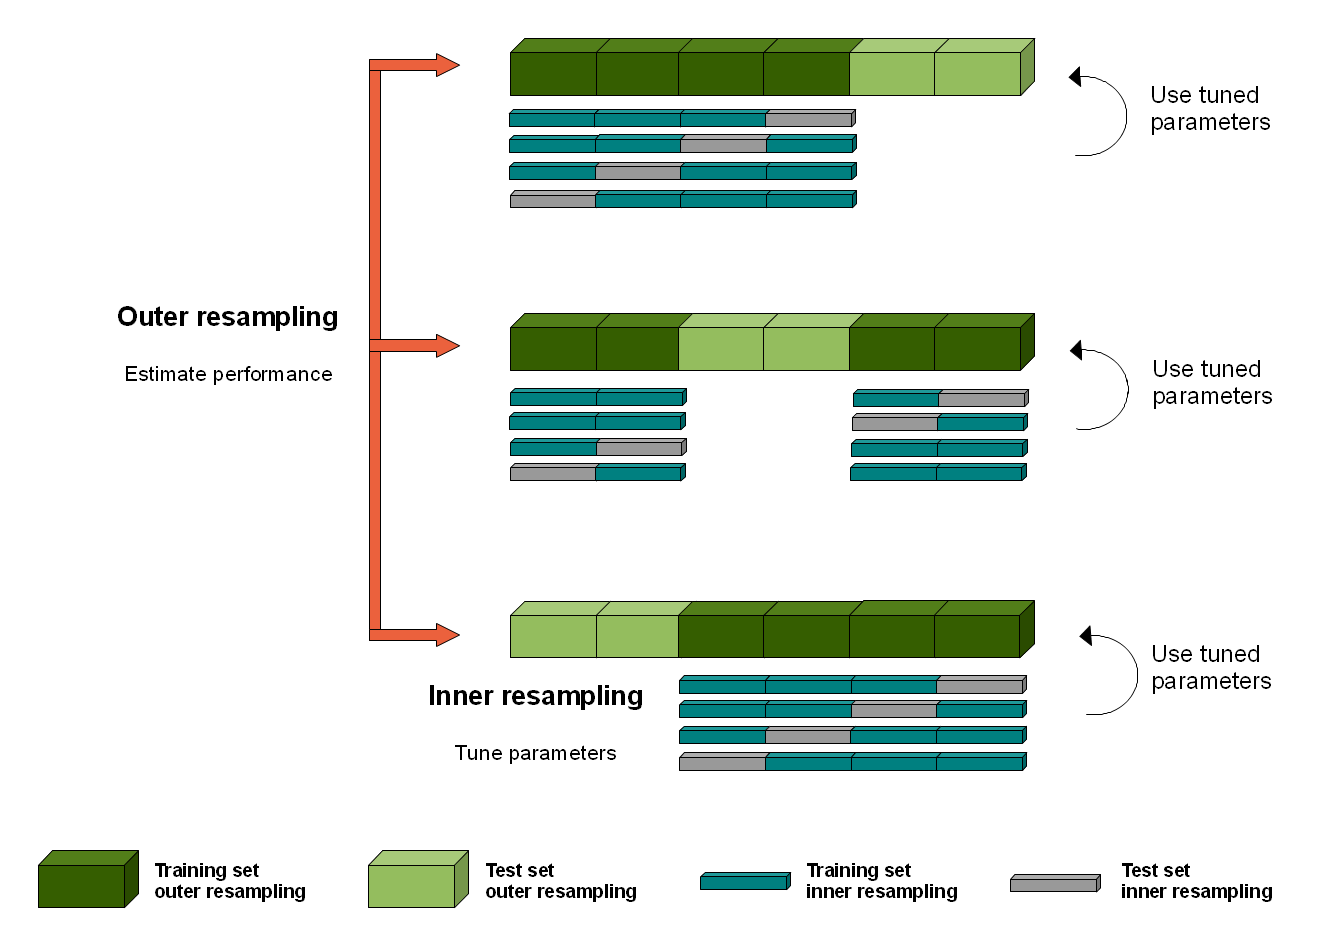
\includegraphics[width = 0.7\textwidth]{figure_man/Nested_Resampling.png}\end{center}

\framebreak

\begin{footnotesize}
In each iteration of the outer loop we:
\begin{itemize}
\item Split off the light green testing data
\item Run the tuner on the dark green part of the data, e.g.,
  evaluate each $\lambda_i$ through fourfold CV on the dark green part
\end{itemize}
\end{footnotesize}

% FIGURE SOURCE: No source
\begin{center}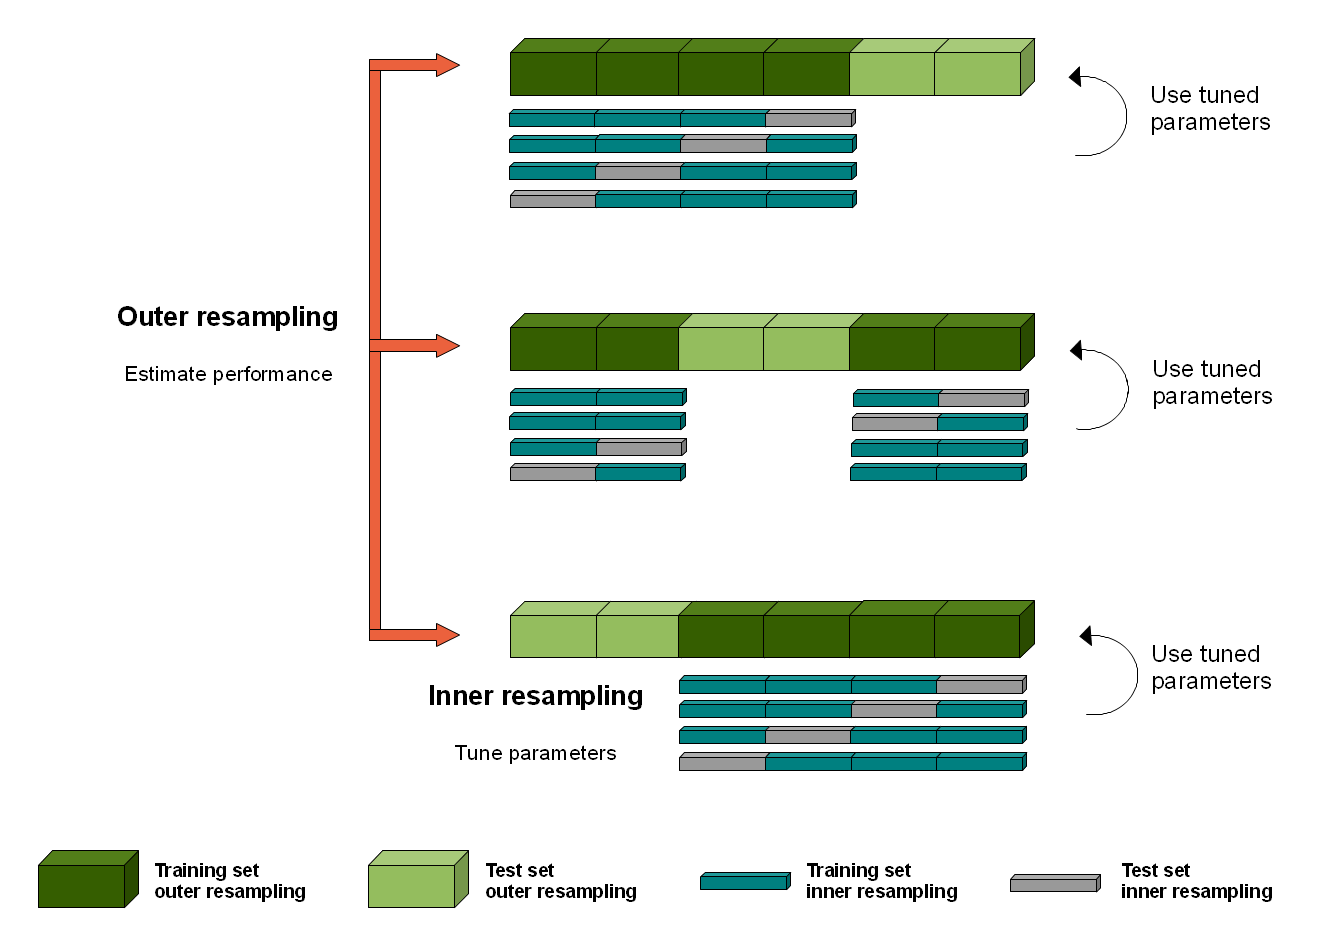
\includegraphics[width = 0.7\textwidth]{figure_man/Nested_Resampling.png}\end{center}

\framebreak

\begin{footnotesize}
In each iteration of the outer loop we:
\begin{itemize}
\item Return the winning $\lambda^*$ that performed best on the grey inner test sets
\item Re-train the model on the full outer dark green train set
\item Evaluate it on the outer light green test set
\end{itemize}
\end{footnotesize}

% FIGURE SOURCE: No source
\begin{center}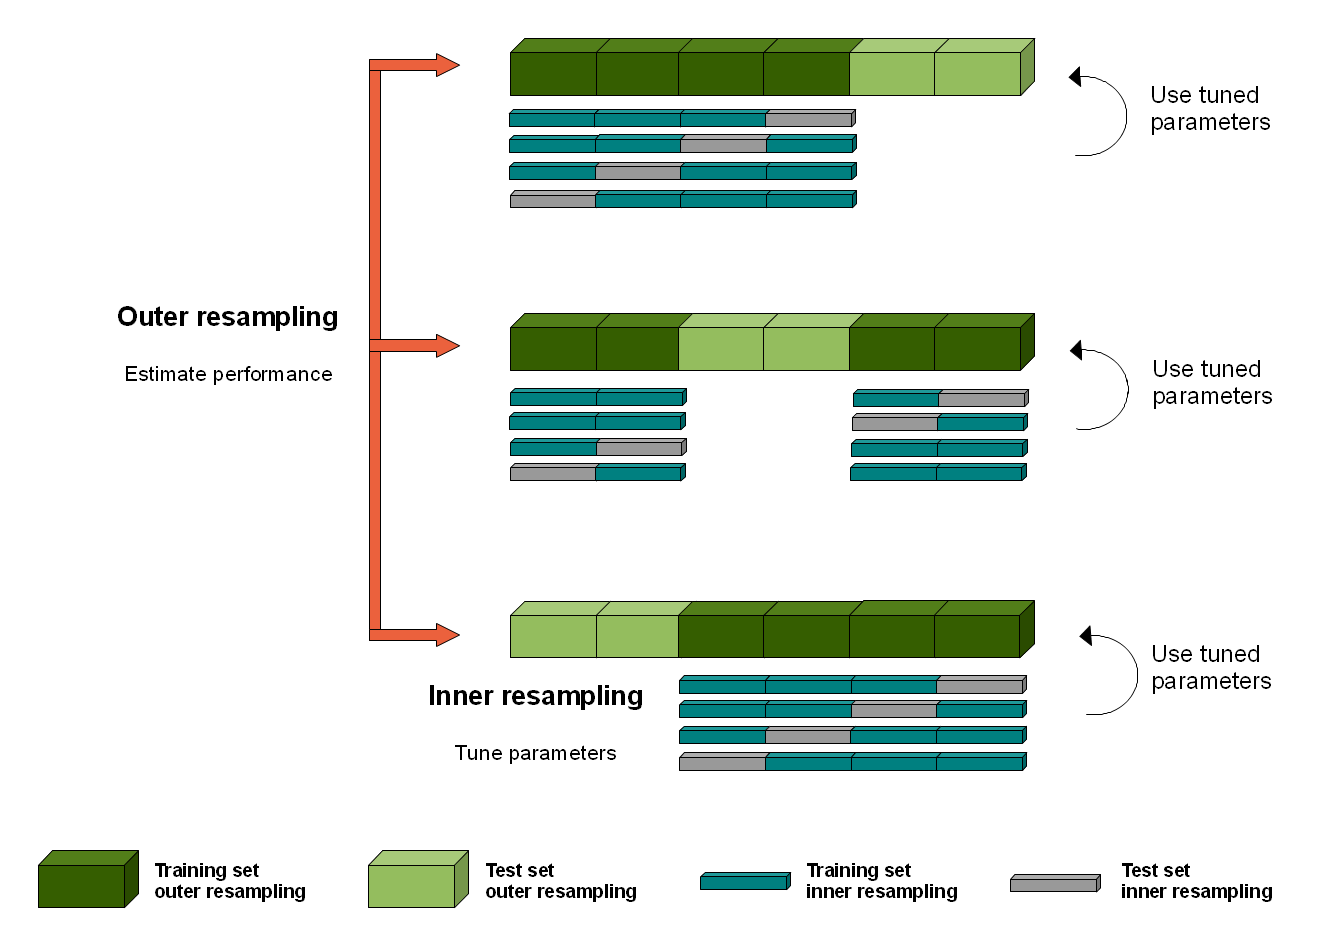
\includegraphics[width = 0.7\textwidth]{figure_man/Nested_Resampling.png}\end{center}

\framebreak

\begin{footnotesize}
The error estimates on the outer samples (light green) are unbiased because this data was strictly excluded from the model-building process of the model that was tested on.
\end{footnotesize}

% FIGURE SOURCE: No source

\begin{center}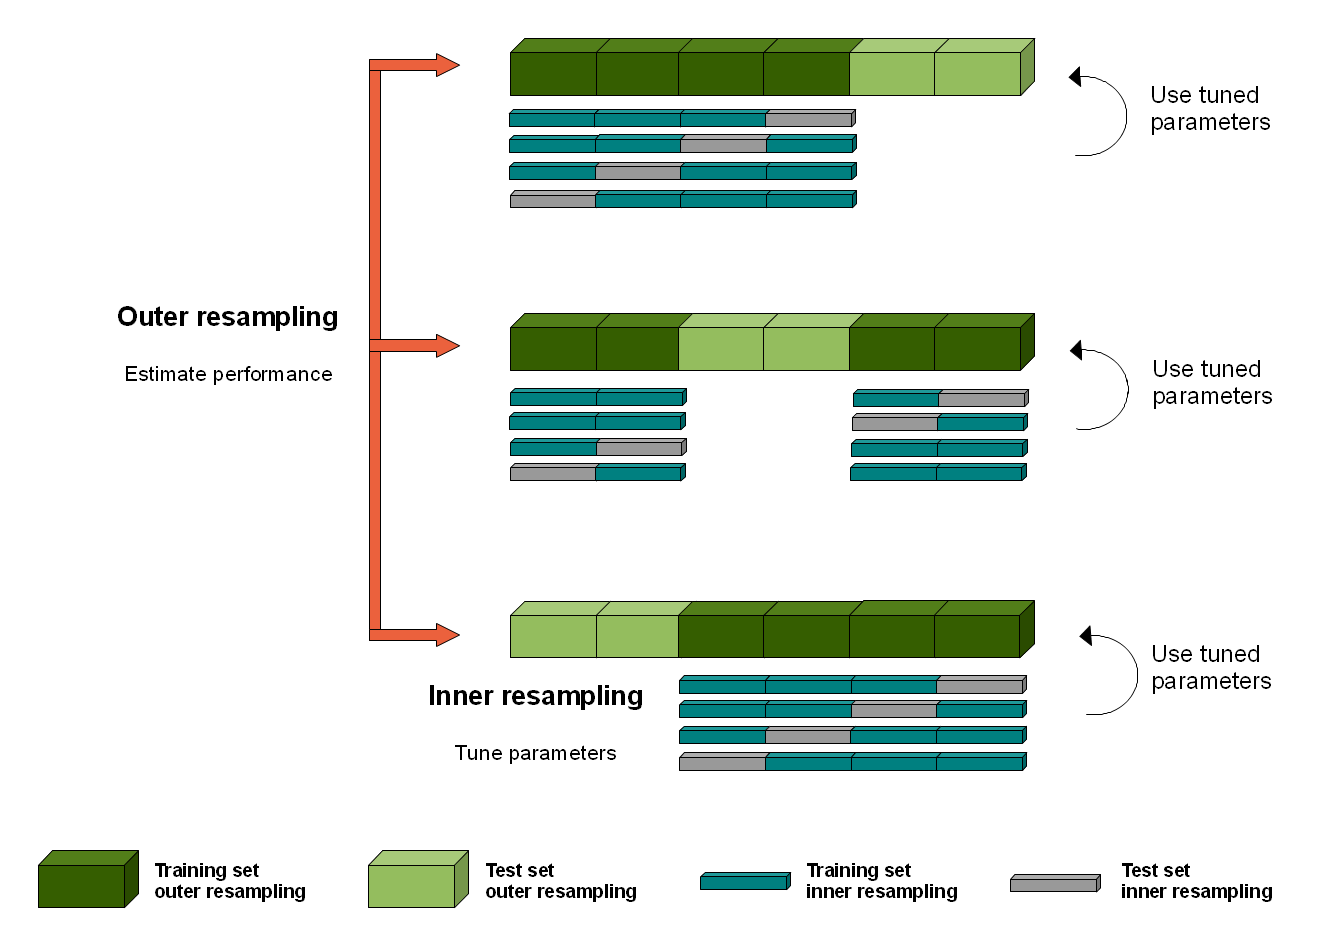
\includegraphics[width = 0.7\textwidth]{figure_man/Nested_Resampling.png}\end{center}

\end{vbframe}



\begin{vbframe}{Nested Resampling - Instructive Example}

Taking again a look at the motivating example and adding a nested resampling outer loop, we get the expected behavior:

\begin{knitrout}\scriptsize
\definecolor{shadecolor}{rgb}{0.969, 0.969, 0.969}\color{fgcolor}

{\centering 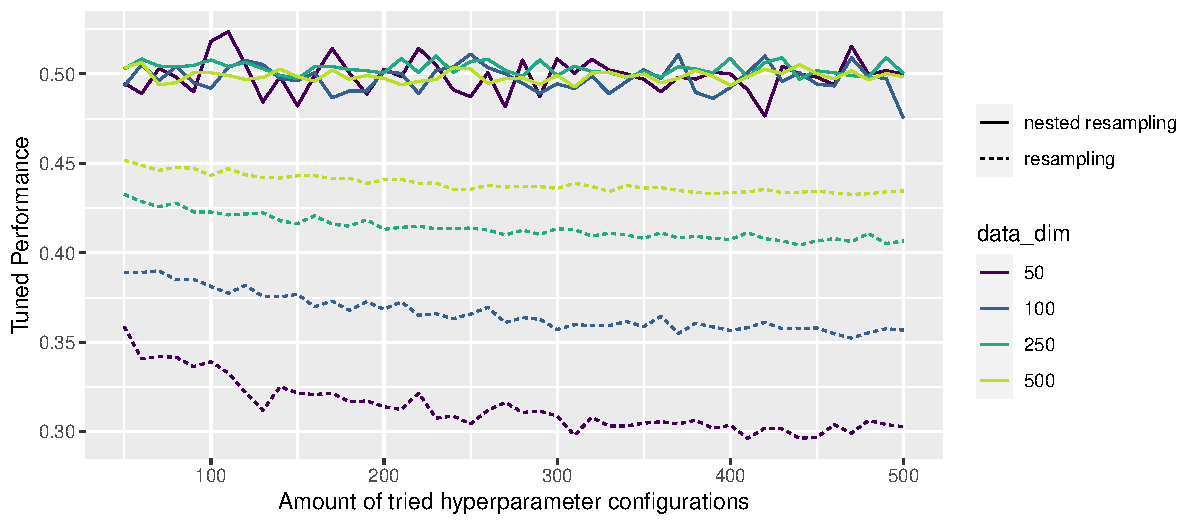
\includegraphics[width=0.95\textwidth]{figure/cart_tuning_nestresample_1} 

}



\end{knitrout}


\end{vbframe}
\endlecture
\end{document}
